\documentclass{beamer}
\usepackage{etex}
\usepackage[utf8]{inputenc}
\usepackage[T1]{fontenc}
\usepackage{amssymb}
\usepackage{color}
\usepackage{verbatim}
\usepackage{beamerthemesplit}
\usepackage{appendixnumberbeamer}
\usepackage{graphicx}
\usepackage{xspace}
\usepackage{algorithm}
\usepackage{listings}
\usepackage{figlatex}
\usepackage{algorithmic}
\usepackage{multirow}
\usepackage{alltt}

\beamertemplatetransparentcovereddynamic

%\setbeamertemplate{background canvas}[vertical shading][bottom=red!10,top=blue!10]
%\usetheme{Warsaw}

\usepackage{../style/beamercolorthemeprogressbar}
\usepackage{../style/beamerfontthemeprogressbar}
\usepackage{../style/beamerouterthemeprogressbar}
\usepackage{../style/beamerinnerthemeprogressbar}

\setbeamertemplate{navigation symbols}{}
\beamertemplatetransparentcovereddynamic

\definecolor{javared}{rgb}{0.6,0,0} % for strings
\definecolor{javagreen}{rgb}{0.30,0.55,0.40} % comments
\definecolor{javapurple}{rgb}{0.5,0,0.35} % keywords
\definecolor{javadocblue}{rgb}{0.25,0.35,0.75} % java


\lstdefinestyle{BOAST}{
  language=Ruby,
  basicstyle=\tiny\ttfamily,
  keywordstyle=\color{javapurple}\bfseries,
  stringstyle=\color{javared},
  commentstyle=\color{javagreen},
  backgroundcolor=\color{white},
  numbers=left,
  morekeywords={BOAST, pr, decl, opn, close, For, Procedure, Real, Int, If, out, inout, Dim}
}
\lstdefinestyle{BFortran}{
  language=Fortran,
  basicstyle=\tiny\ttfamily,
  keywordstyle=\color{javapurple}\bfseries,
  stringstyle=\color{javared},
  commentstyle=\color{javagreen},
  numbers=left,
  tabsize=4,
  showspaces=false,
  showstringspaces=false
}
\lstdefinestyle{BC}{
  language=C,
  basicstyle=\tiny\ttfamily,
  keywordstyle=\color{javapurple}\bfseries,
  stringstyle=\color{javared},
  commentstyle=\color{javagreen},
  numbers=left,
  tabsize=4,
  showspaces=false,
  showstringspaces=false,
  morekeywords={kernel, global, uchar, short16, uchar16, int16, int32\_t, int64\_t},
}

\graphicspath{{../figures/}}

\title{BOAST}
\subtitle{A Computing Kernel Metaprogramming and Autotuning Framework for Heterogeneous Architectures}
\author[B. V.]{\textbf{Brice~Videau}~\inst{1}, Kevin~Pouget~\inst{2}, Luigi~Genovese~\inst{3},
                    Thierry~Deutsch~\inst{3}, Julien Bigot~\inst{3}, Guillaume Latu~\inst{3}, Virginie Grandgirard~\inst{3}, Dimitri~Komatitsch~\inst{4}, Fr\'ed\'eric~Desprez~\inst{2}, Jean-François~Méhaut~\inst{2}}
\institute[ANL]{
\inst{1} ANL,
\inst{2} INRIA/LIG,
\inst{3} CEA,
\inst{4} CNRS
}

\date{\textbf{SIAMPP22} - Minisymposium on Code Generation and Transformation in HPC on Heterogeneous Platforms\\February 26, 2022}

%\logo{
%   
\includegraphics[scale=.09]{logo_eocoe}
%   }

\bibliographystyle{plain}
\begin{document}

\frame{\titlepage}

\section{Introduction}

\subsection{Context}

\begin{frame}
  \frametitle{Scientific Application Portability}

  \begin{block}{\footnotesize Limited Portability}
    \begin{itemize}
      \item \scriptsize Huge codes (more than 100 000 lines), Written in FORTRAN or C++
      \item \scriptsize Collaborative efforts
      \item \scriptsize Use many different programming paradigms (OpenMP, OpenCL, CUDA, ...)
    \end{itemize}
  \end{block}

  \begin{columns}

  \column{0.45\linewidth}
  \begin{block}{\footnotesize But Based on \emph{Computing Kernels}}
    \begin{itemize}
      \item \scriptsize Well defined parts of a program
      \item \scriptsize Compute intensive
      \item \scriptsize Prime target for optimization
    \end{itemize}
  \end{block}

  \column{0.58\linewidth}
  \begin{block}{\footnotesize Kernels Should Be Written}
    \begin{itemize}
      \item \scriptsize In a \emph{portable} manner
      \item \scriptsize In a way that raises developer \emph{productivity}
      \item \scriptsize To present good \emph{performance}
    \end{itemize}
  \end{block}

  \end{columns}

\end{frame}

\subsection{Related Work}

\begin{frame}
  \frametitle{Related Work}

  \begin{itemize}
    \item \textbf{Ad hoc autotuners (usually for libraries):}
    \begin{itemize}
      \item \textbf{Atlas}~\cite{whaley04} (C macro processing)
      \item \textbf{SPIRAL}~\cite{puschel2004spiral} (DSL)
      \item ...
    \end{itemize}
    \item \textbf{Generic frameworks using annotation systems:}
    \begin{itemize}
      \item \textbf{POET}~\cite{yi2007poet} (external annotation file)
      \item \textbf{Orio}~\cite{Hart2009:Orio} (source annotation)
      \item \textbf{BEAST}~\cite{CPE:CPE3516} (Python preprocessor based, embedded DSL for optimization space definition/pruning)
    \end{itemize}
    \item \textbf{Generic frameworks using embedded DSL:}
    \begin{itemize}
      \item \textbf{Halide}~\cite{ragan2013halide} (C++, not very generic, 2D stencil targeted)
      \item \textbf{Heterogeneous Programming Library}~\cite{F.Fabeiro:2016:WPM:2894387.2894576} (C++)
    \end{itemize}
  \end{itemize}

\end{frame}

\section{A Parametrized Generator}
\begin{frame}
\frametitle{BOAST: a Parametrized Generator}
\end{frame}

\subsection{Motivation and Principles}

\begin{frame}

  \frametitle{Classical Tuning of Computing Kernels}

  \begin{center}%
    \includegraphics<1>[scale=1]{Workflow1-1}%
    \includegraphics<2>[scale=1]{Workflow1-2}%
    \includegraphics<3>[scale=1]{Workflow1-3}%
    \includegraphics<4>[scale=1]{Workflow1-4}%
  \end{center}%
  \begin{itemize}%
\only<1>{    \item Kernel optimization workflow}%
\only<1>{    \item Usually performed by a knowledgeable developer}%
\only<2>{    \item Compilers perform optimizations}%
\only<2>{    \item Architecture specific or generic optimizations}%
\only<3>{    \item Performance data hint at source transformations}%
\only<3>{    \item Architecture specific or generic hints}%
\only<4>{    \item Multiplication of kernel versions and/or loss of versions}%
\only<4>{    \item Difficulty to benchmark versions against each-other}%
  \end{itemize}%

\end{frame}

\begin{frame}
  \frametitle{BOAST Workflow \vphantom{Cp}}
  \begin{center}
    \includegraphics<1>[scale=1]{Workflow2-1}
    \includegraphics<2>[scale=1]{Workflow2-2}
    \includegraphics<3>[scale=1]{Workflow2-3}
  \end{center}
  \begin{itemize}%
\only<1>{    \item Meta-programming of optimizations in BOAST }
\only<1>{    \item High level object oriented language }
\only<2>{    \item Generate combination of optimizations }
\only<2>{    \item C, OpenCL, FORTRAN and CUDA are supported }
\only<3>{    \item Compilation and analysis are automated }
\only<3>{    \item Selection of best version can also be automated \vphantom{Cp}}
  \end{itemize}%
\end{frame}

\begin{frame}
\frametitle{BOAST Architecture}
 \begin{center}
   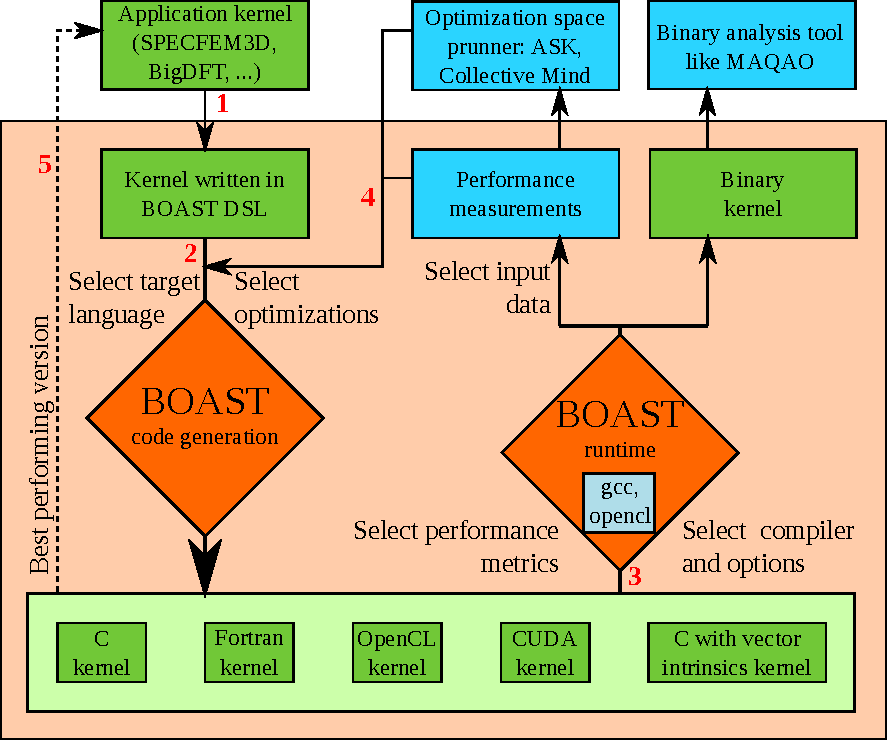
\includegraphics[scale=0.5]{BOAST_Workflow}
 \end{center}
\end{frame}

\subsection{Simple Illustration}

\begin{frame}[fragile]
\frametitle{Kernel Definition}
\lstset{style=BOAST}
\begin{lstlisting}
require 'narray'
require 'BOAST'
include BOAST

set_array_start(0)
set_default_real_size(4)

def vector_add
  n = Int("n",:dir => :in)
  a = Real("a",:dir => :in, :dim => [ Dim(n)] )
  b = Real("b",:dir => :in, :dim => [ Dim(n)] )
  c = Real("c",:dir => :out, :dim => [ Dim(n)] )
  p = Procedure("vector_add", [n,a,b,c]) {
    decl i = Int("i")
    expr = c[i] === a[i] + b[i]
    if (get_lang == CL or get_lang == CUDA) then
      pr i === get_global_id(0)
      pr expr
    else
      pr For(i,0,n-1) {
        pr expr
      }
    end
  }
  return p.ckernel
end
\end{lstlisting}
\end{frame}

\begin{frame}[fragile]
\frametitle{Kernel Testing}
\lstset{style=BOAST}
\begin{lstlisting}
n = 1024*1024
a = NArray.sfloat(n).random!
b = NArray.sfloat(n).random!
c = NArray.sfloat(n)
c_ref = a + b

epsilon = 1e-8

[FORTRAN, C, CL, CUDA].each { |l|
  set_lang( l )
  puts "#{get_lang_name}:"
  k = vector_add
  puts k
  c.random!
  puts k.run(n, a, b, c, global_work_size: [n,1,1], local_work_size: [32,1,1])
  diff_max = (c_ref - c).abs.max
  raise "Error: max error too big: #{diff_max}!" if diff_max > epsilon
}
puts "Success!"
\end{lstlisting}
\end{frame}


\subsection{Evaluation}

\begin{frame}
\frametitle{Strength and Weakness of the Approach}
Major benefits:
\begin{itemize}
\item Powerful meta-programming capabilities, Ruby is your macro-processor;
\item Generated kernels are readable, can be debugged, and can be integrated in applications;
\item Kernel correctness and performance evaluation is efficient:
  \begin{itemize}
  \item Kernels are self contained,
  \item and ran inside BOAST memory space, avoiding repeated setup.
  \end{itemize}
\end{itemize}
Major hurdles:
\begin{itemize}
\item Upfront cost of kernel extraction and setting up validation can be important if data shape is complex;
\item Debugging syntax errors in lambdas can be difficult;
\item No semantic validation beside basic type checking;
\end{itemize}

\end{frame}

\section{Case Studies}

\begin{frame}
\frametitle{Case Studies}
\end{frame}

\subsection{BigDFT}

\begin{frame}
  \frametitle{BigDFT}
  \begin{center}
    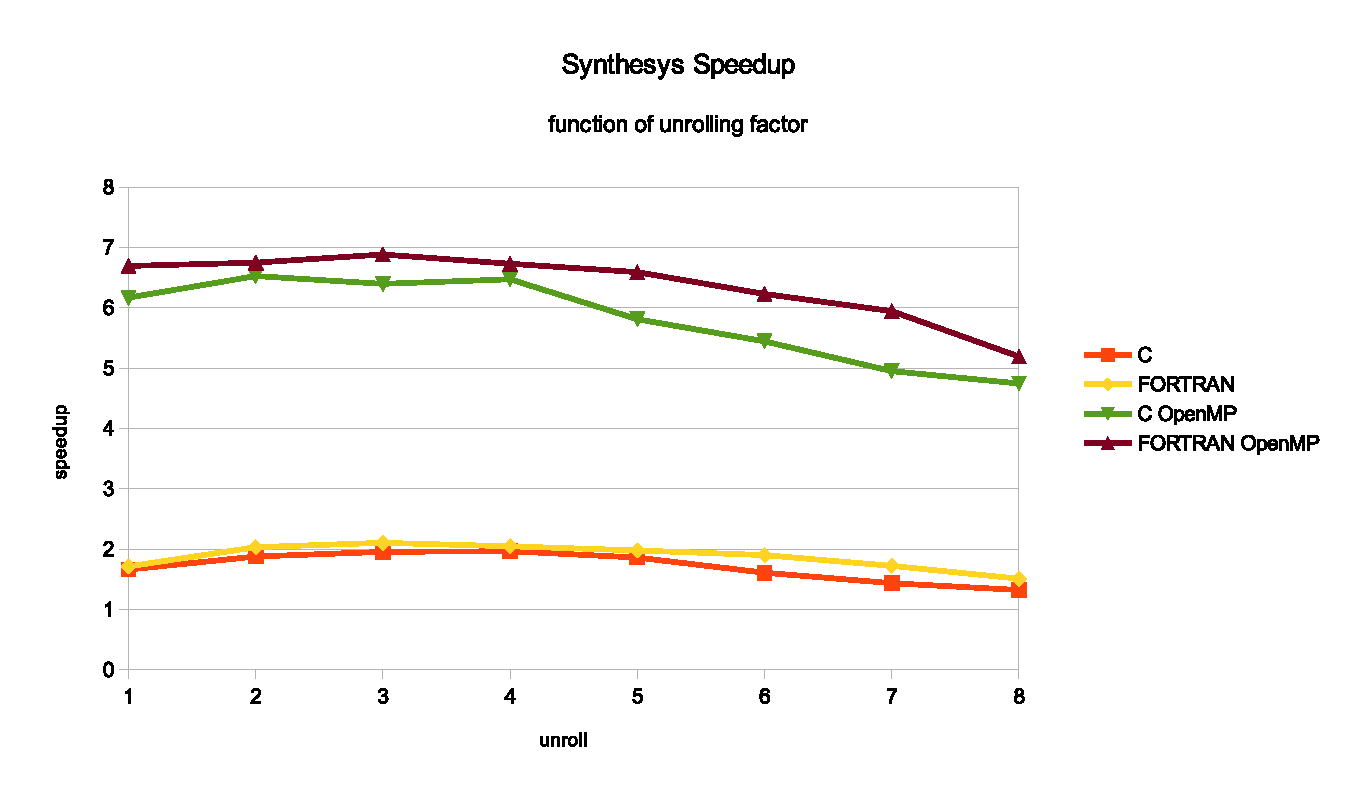
\includegraphics[scale=0.35]{Res_synthesis}
  \end{center}

 \begin{itemize}
  \item Novel approach for DFT computation based on Daubechies wavelets
  \item Fortran and C code, MPI, OpenMP, supports CUDA and OpenCL
  \item Reference is hand tuned code on target architecture (Nehalem)
  \item BLAS-like library for wavelets: \url{https://github.com/luigigenovese/libconv}
  \end{itemize}
\end{frame}

\subsection{SPECFEM3D}

\begin{frame}
  \frametitle{SPECFEM3D}

  \begin{itemize}
   \item Seismic wave propagation simulator
    \item SPECFEM3D ported to OpenCL using BOAST, and now HIP
    \begin{itemize}
      \item Unified code base (CUDA/OpenCL/HIP)
      \item Refactoring: kernel code base reduced by 40\%
      \item Similar performance on NVIDIA Hardware
      \item Non regression test for GPU kernels
    \end{itemize}
    \item On the Mont-Blanc prototype:
    \begin{itemize}
      \item OpenCL+MPI runs
      \item Speedup of 3 for the GPU version
    \end{itemize}
  \end{itemize}
\end{frame}

\subsection{Laplacian Filter}

\begin{frame}[fragile]
  \frametitle{Laplace Kernel Port to ARM Mali GPU - 1}
\lstset{style=BC}
\begin{lstlisting}
void laplace(const int width,
             const int height,
             const unsigned char src[height][width][3],
                   unsigned char dst[height][width][3]){
  for (int j = 1; j < height-1; j++) {
    for (int i = 1; i < width-1; i++) {
      for (int c = 0; c < 3; c++) {
        int tmp = -src[j-1][i-1][c] -   src[j-1][i][c] - src[j-1][i+1][c]\
                 - src[j  ][i-1][c] + 9*src[j  ][i][c] - src[j  ][i+1][c]\
                 - src[j+1][i-1][c] -   src[j+1][i][c] - src[j+1][i+1][c];
        dst[j][i][c] = (tmp < 0 ? 0 : (tmp > 255 ? 255 : tmp));
      }
    }
  }
}
\end{lstlisting}
\begin{itemize}
\item C reference implementation
\item Many possible optimization strategies in OpenCL
\item ARM GPU Mali 604 within the Mont-Blanc project
\end{itemize}
\end{frame}

\begin{frame}
  \frametitle{Laplace Kernel Port to ARM Mali GPU - 2}
  Hand tuned code by specialist uses vectorization, temporary data-type change, and register swizzling to avoid loads
  \begin{columns}
  \column{0.55\textwidth}
  \begin{itemize}
    \item Hyperparameters used in BOAST:
    \begin{itemize}
      \item \emph{tile\_x}: a positive integer
      \item \emph{tile\_y}: a positive integer
      \item \emph{vector\_length}: 1, 2, 4, 8 or 16
      \item \emph{temporary\_size}: 2 or 4 bytes
      \item \emph{register\_swizzle}: true or false
    \end{itemize}
  \end{itemize}
  \column{0.45\textwidth}
  \begin{itemize}
    \item Optimal parameter values:
    \begin{itemize}
      \item tile\_x: 16
      \item tile\_y: 1
      \item vector\_length: 16
      \item temporary\_size: 2
      \item register\_swizzle: \emph{false}
    \end{itemize}
  \end{itemize}
  \end{columns}

  \begin{center}
  \scriptsize
  \begin{tabular}{c|r|r|c|r|c}
    Image Size  & Naive (s) & Best (s) & Acceleration & BOAST (s) & Acceleration \\
    \hline&&&&\\
  768 x 432   & 0.0107    & 0.00669  & x1.6         & 0.000639  & x16.7 \\
  2560 x 1600 & 0.0850    & 0.0137   & x6.2         & 0.00687   & x12.4 \\
  2048 x 2048 & 0.0865    & 0.0149   & x5.8         & 0.00715   & x12.1 \\
  5760 x 3240 & 0.382     & 0.0449   & x8.5         & 0.0325    & x11.8 \\
  7680 x 4320 & 0.680     & 0.0747   & x9.1         & 0.0581    & x11.7
  \end{tabular}
  \end{center}

\end{frame}

\begin{frame}
  \frametitle{Laplace Kernel Port to ARM Mali GPU - 3}
  \begin{center}
  \scriptsize
  \begin{tabular}{c|r|r|c|r|c}
    Image Size & BOAST ARM (s) & BOAST Intel & Ratio & BOAST NVIDIA & Ratio \\
    \hline&&&&\\
  768 x 432   & 0.000639     & 0.000222    & x2.9  & 0.0000715    & x8.9  \\
  2560 x 1600 & 0.00687      & 0.00222     & x3.1  & 0.000782     & x8.8  \\
  2048 x 2048 & 0.00715      & 0.00226     & x3.2  & 0.000799     & x8.9  \\
  5760 x 3240 & 0.0325       & 0.0108      & x3.0  & 0.00351      & x9.3  \\
  7680 x 4320 & 0.0581       & 0.0192      & x3.0  & 0.00623      & x9.3
  \end{tabular}
  \end{center}

  \begin{columns}
  \column{0.5\textwidth}
  \begin{itemize}
    \item \footnotesize Optimal parameter values Intel\\(I7 2760):
    \begin{itemize}
      \item \scriptsize tile\_x: 16
      \item \scriptsize tile\_y: 4..2
      \item \scriptsize vector\_length: 8
      \item \scriptsize temporary\_size: 2
      \item \scriptsize register\_swizzle: false
    \end{itemize}
  \end{itemize}
  \column{0.5\textwidth}
  \begin{itemize}
    \item \footnotesize Optimal parameter values nVidia\\(GTX 680):
    \begin{itemize}
      \item \scriptsize tile\_x: 4
      \item \scriptsize tile\_y: 4
      \item \scriptsize vector\_length: 4
      \item \scriptsize temporary\_size: 2
      \item \scriptsize register\_swizzle: false
    \end{itemize}
  \end{itemize}
  \end{columns}
  \vspace{1cm}
  \centering Performance \emph{portability} among several different architectures.
\end{frame}

\subsection{Gysela}

\begin{frame}
\frametitle{Gysela 2d avection}

\scalebox{1.}{
\begin{minipage}{\textwidth}
Gysela: Gyrokinetic Semi-Lagrangian\\
Tokamak plasma simulation for fusion (ITER)
\begin{itemize}
\item Chosen Auto-tuning parameters:
\begin{itemize}
\item directive based inlining / BOAST driven inlining
\item BOAST driven loop unrolling
\item C or Fortran code generated
\item scan versions of gfortran/gcc/icc/ifort
\item loop blocking parameter (one of the most internal loop)
\item explicit vectorization: BOAST generates INTEL intrinsincs, e.g.
\scalebox{.6}{
\begin{minipage}{1.5\textwidth}
\begin{alltt}
ftmp1 = \_mm256\_setzero\_pd( );\\
ftmp2 = \_mm256\_setzero\_pd( );\\
ftmp1 = \_mm256\_fmadd\_pd(  base1[0], \_mm256\_load\_pd( \&ftransp[(0) * (4)]);\\
ftmp2 = \_mm256\_fmadd\_pd( base1[0 + 1], \_mm256\_load\_pd( \&ftransp[(0 + 1)  * (4)] ), ftmp2 );
\end{alltt}
\end{minipage}}
\end{itemize}
\item Final result: Ruby code of 200 lines for the 2d advection kernel (vs 300 original FORTRAN)
\item between 1 min and 20 min for the {parameter scan} on 1 machine
\end{itemize}
\end{minipage}}

\end{frame}

\begin{frame}
\frametitle{Auto-tuning on INTEL Westmere (2011)}
\begin{columns}
\column{.3\textwidth}
\scalebox{0.76}{
\begin{minipage}{6cm}
Auto-tuning for 2D advection\\
Computing center at Marseille\\
12-cores node -\\
\hspace*{.4cm} Intel X5675, 3.07GHz\\[1cm]
Nb of runs in this scan: 609\\
Runs sorted from quickest to slowest\\
Result of the scan \\
\hspace*{.4cm}\ (best parameters):\\[.2cm]
\end{minipage}
}
\scalebox{0.7}{
\begin{minipage}{6cm}
\begin{alltt}
:lang: FORTRAN\\
:unroll: true\\
:force.inline: true\\
:intrinsic: false\\
:blocking.size: 4\\
:module: intel/16.0.2\\
\end{alltt}

Speedup: \textcolor{red}{1.9}
\end{minipage}
}
\column{.70\textwidth}
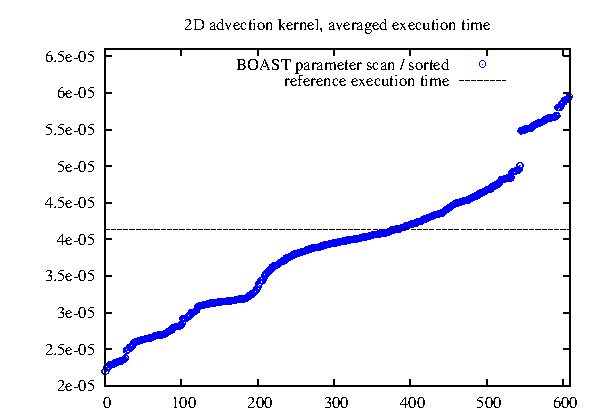
\includegraphics[width=1.0\textwidth]{rheticus.pdf}\\
\end{columns}
\end{frame}
  
\begin{frame}
\frametitle{Auto-tuning on INTEL Sandy-Bridge (2012)}
\begin{columns}
\column{.3\textwidth}
\scalebox{0.8}{
\begin{minipage}{6cm}
Auto-tuning for 2D advection\\
Computing center at Orsay\\
16-cores node - \\
\hspace*{0.4cm}Intel E5-2670 v1, 2.60GHz\\[1cm]
Result of the scan \\
\hspace*{.4cm}\ (best parameters):\\[.2cm]
\end{minipage}
}
\scalebox{0.7}{
\begin{minipage}{6cm}
\begin{alltt}
:lang: FORTRAN\\
:unroll: \textcolor{red}{false}\\
:force.inline: \textcolor{red}{false}\\
:intrinsic: false\\
:blocking.size: 2\\
:module: intel/15.0.0
\end{alltt}

Speedup: \textcolor{red}{1.7}
\end{minipage}
}
\column{.70\textwidth}
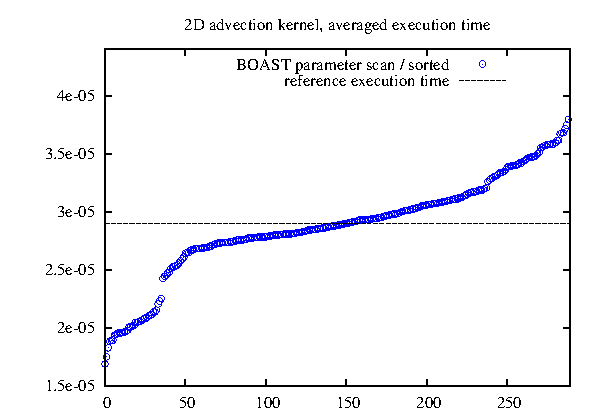
\includegraphics[width=1.0\textwidth]{poincare.pdf}\\
\end{columns}
\end{frame}
  
\begin{frame}
\frametitle{Auto-tuning on INTEL Haswell (2015)}
\begin{columns}
\column{.3\textwidth}
\scalebox{0.8}{
\begin{minipage}{6cm}
Auto-tuning for 2D advection\\
Computing center at Montpellier\\
24-cores node - \\
\hspace*{0.4cm}Intel E5-2690 v3, 2.60GHz\\[1cm]
Result of the scan \\
\hspace*{.4cm}\ (best parameters):\\[.2cm]
\end{minipage}
}
\scalebox{0.7}{
\begin{minipage}{6cm}
\begin{alltt}
:lang: FORTRAN\\
:unroll: true\\
:force.inline: true\\
:intrinsic: false\\
:blocking.size: 4\\
:module: \textcolor{red}{intel/14.0.4.211}\\
\end{alltt}

Speedup: \textcolor{red}{2.0}
\end{minipage}
}
\column{.70\textwidth}
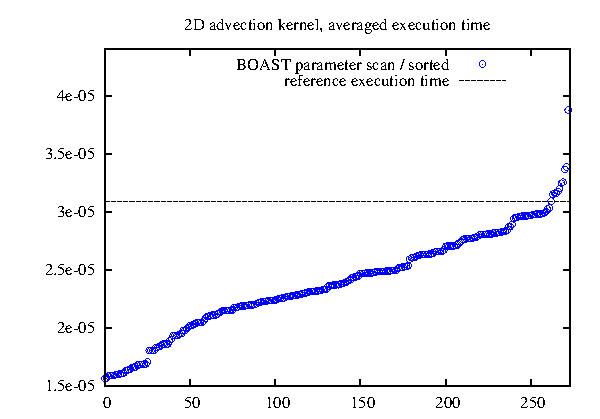
\includegraphics[width=1.0\textwidth]{occigen.pdf}\\
\end{columns}
\end{frame}

\begin{frame}
\frametitle{Auto-tuning on INTEL KNL (Phi 2016)}
\begin{columns}
\column{.3\textwidth}
\scalebox{0.8}{
\begin{minipage}{6cm}
Auto-tuning for 2D advection\\
Computing center at Montpellier\\
64-cores node - \\
\hspace*{0.4cm}Intel 7210  1.30GHz\\[1cm]
Result of the scan \\
\hspace*{.4cm}\ (best parameters):\\[.2cm]
\end{minipage}
}
\scalebox{0.7}{
\begin{minipage}{6cm}
\begin{alltt}
:lang: FORTRAN\\
:unroll: true\\
:force.inline: true\\
:intrinsic: false\\
:blocking.size: \textcolor{red}{32}\\
:module: \textcolor{red}{intel/17.0}\\
\end{alltt}

Speedup: \textcolor{red}{3.6}
\end{minipage}
}
\column{.70\textwidth}
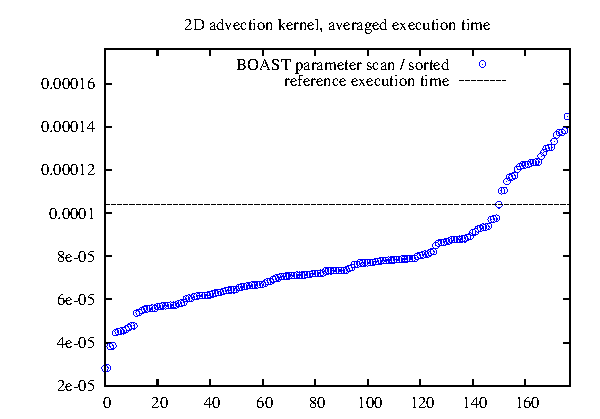
\includegraphics[width=1.0\textwidth]{knl.pdf}\\
\end{columns}
\end{frame}

\begin{comment}
\section{Real Applications}
\end{comment}

\section{Conclusion}

\begin{frame}
\frametitle{Conclusion}
\end{frame}

\begin{frame}
  \frametitle{Conclusion}
  \begin{itemize}
    \item A kernel tuning framework based on code transformation and generation proved:
    \begin{itemize}
      \item Flexible enough to cover a broad range of applications and targets,
      \item While still outperforming hand tuned or other compiler based optimization strategies,
      \item Maintainable as BOAST is still used in production after a decade.
    \end{itemize}
    \item But also useful for:
    \begin{itemize}
      \item Auto-tuning research,
      \item Architecture and compiler performance evaluation,
      \item Non-regression testing through kernel replay and validation.
    \end{itemize}
  \end{itemize}
  Hopefully, this approach (if not BOAST itself) will be picked up in the future and further generalized and improved.
\end{frame}

\appendix
\subsection{Bibliography}

\begin{frame}[shrink=50]
  \frametitle{Bibliography}
  \bibliography{../biblio/BOAST}
\end{frame}

\subsection{Acknowledgements}
\begin{frame}
  \frametitle{Acknowledgements}
  \begin{itemize}
    \item This project has received funding from the European Union's Horizon 2020 research and innovation programme under grant agreement Nos 288777, 610402, and EINFRA-676629
    \item The research leading to these results has received funding from the European Union’s Horizon 2020 Programme (2014-2020) and from Brazilian Ministry of Science, Technology and Innovation through Rede Nacional de Pesquisa (RNP) under the HPC4E project, grant agreement No 689772
    \item This research used resources of the Argonne Leadership Computing Facility, which is a DOE Office of Science User Facility supported under Contract DE-AC02-06CH11357.
  \end{itemize}
\end{frame}

\end{document}
